%*********************************************************************************
\subsection{Simulation Experiment}\label{sub:sa_application_simulation_experiment}
%*********************************************************************************

The simulation experiment was carried out in two steps.
The first step was aimed at screening out any possible noninfluential parameters using several screening methods, 
while the second step consisted of estimating the Sobol' sensitivity indices on the reduced number of parameters.
The screening methods considered here are two variants of the Morris screening method (the radial and the trajectory designs) and the Sobol'-Saltelli method to estimate the total-effect indices.
Since the number of parameters is directly proportional to the number of code runs, 
the screening procedure done in the first step allowed us to generate a larger sample for fewer code runs to make the \gls[hyper=false]{mc} estimates of the Sobol' indices more precise.
Note that the total duration of the transient is set to be $600 \ [s]$ and each TRACE run required between $\sim 400$ and $600 \ [CPUs]$.

The experimental design matrix used to carry out the estimation was generated using a Sobol' quasi-random sequence generator \cite{Joe2008} (See Appendix~\ref{app:doe} for more detail).
The flowchart of the simulation experiment for the analysis is illustrated and summarized in Fig.~\ref{fig:sensitivity_flowchart}.

\begin{sidewaysfigure}
	\centering
	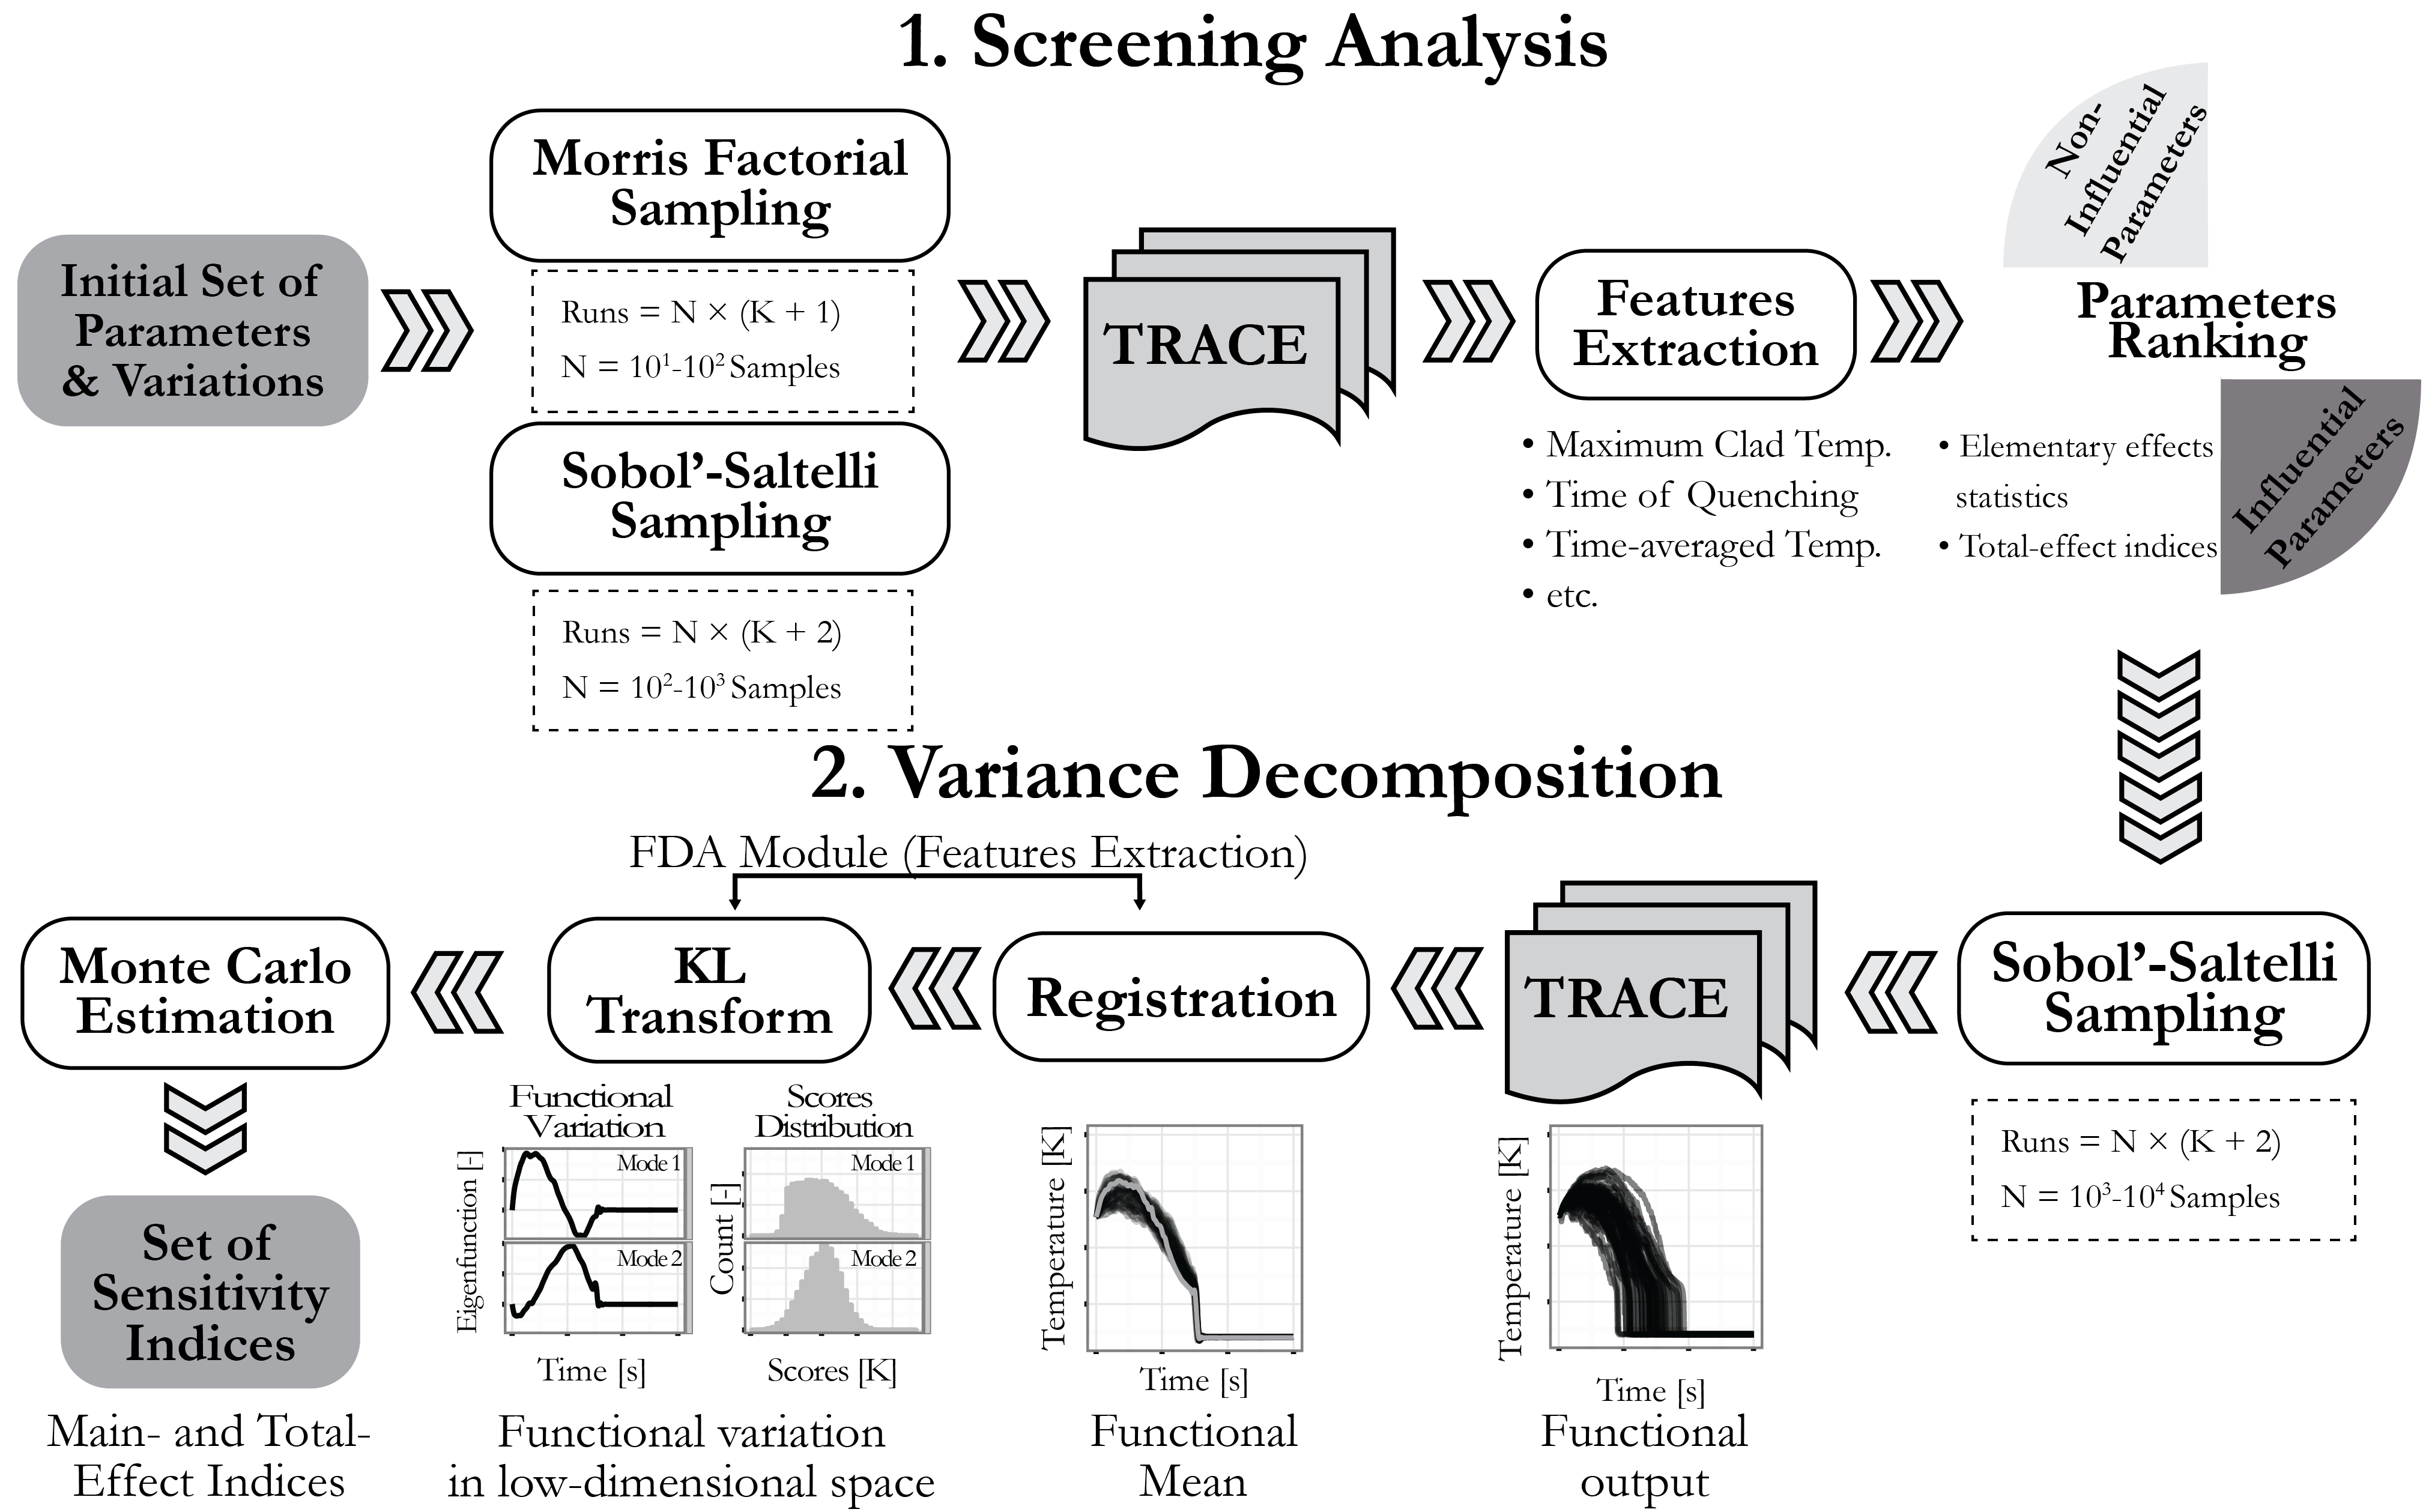
\includegraphics[width=0.85\textwidth]{../figures/chapter3/ai/simulation_experiment.png}
	\caption[The flowchart for the implemented sensitivity analysis methodology applied to the TRACE model of FEBA facility]{The flowchart for the implemented sensitivity analysis methodology applied to the \gls[hyper=false]{trace} model of \gls[hyper=false]{feba} facility.}
	\label{fig:sensitivity_flowchart}
\end{sidewaysfigure}

Different types of \glspl[hyper=false]{qoi} have been investigated for this simulation experiment.
The application of the Morris method to the TRACE model of the FEBA facility to rank the parameter importance was already demonstrated in \cite{Wicaksono2014} using the time-averaged temperature as QoI, 
which is defined as
\begin{equation}
	\bar{T} = \frac{\int T(t) dt}{\int dt}
\label{eq:qoi_time_averaged_temperature}
\end{equation}
where the integration of the pointwise time-dependent reflood curve was approximated using the trapezoidal rule over the duration of the transient.
The time-averaged temperature was selected as the simplest possible scalar \gls[hyper=false]{qoi} to capture the overall variation of the temperature transient 
since it was previously shown that a high maximum cladding temperature as \gls[hyper=false]{qoi} would not necessarily imply later quench time, and vice versa \cite{Wicaksono2014}. 
To further investigate these aspects, the maximum cladding temperature and the quench time have also been considered as \glspl[hyper=false]{qoi} in this study.

The derivation of more innovative \glspl[hyper=false]{qoi} necessitated the analysis of the transient output samples using \gls[hyper=false]{fda} techniques.
All the steps required in the \gls[hyper=false]{fda} were already demonstrated in the context of the reflood simulation output in \cite{Wicaksono2014a}.
All the required computations related to \gls[hyper=false]{fda} were done in \texttt{R} programming language and statistical computing environments \cite{RCT2017} using the \texttt{fda} package \cite{Ramsay2014}.

The resulting principal component score for each realization was therefore used as the \gls[hyper=false]{qoi} for the Sobol' indices calculation and compared to the indices obtained from the more conventional \glspl[hyper=false]{qoi} for the reflood transient.
Finally, to give a measure of the uncertainty in the all indices estimated by \gls[hyper=false]{mc} procedure, 
the $95$\% percentile \gls[hyper=false]{ci} were constructed using the bootstrap technique (\cite{Efron1986} and see Appendix.~\ref{app:bootstrapping} for detail).
